% Provenance (never printed): see sources/outline_sources.md (Year 1: rigid plates on a
% sphere, Euler poles and angular velocities; relative velocities; triple junctions;
% finite rotations; the magnetic-anomaly timescale; satellite geodesy). Curves and maps
% from figdata/bachelor-1/euler_velocities.py, south_atlantic_fit.py and gpts_stripes.py;
% exercise and problem values in the Book 3 scratch calculator calc/ch12.py.
\chapter{Cinématique des plaques sur une sphère}\label{ch:b1:plate-kinematics}

Deux stations de positionnement par satellite enregistrent leur position chaque
jour depuis plus d'un quart de siècle~: l'une à Reykjavik, dans l'ouest de
l'Islande, l'autre près de Stavanger, sur la côte ouest de la Norvège. La droite
qui les joint, longue de \qty{1546}{km}, s'allonge de \qty{17.5}{mm} chaque année,
près de deux centimètres. Rien ne le montre sur le terrain, et pourtant le plancher du
nord de l'Atlantique entre les deux stations enregistre le même élargissement sur
des millions d'années~: la lave émise à la dorsale médio-atlantique a pris la
direction du champ magnétique terrestre en se refroidissant, et le champ s'est inversé
bien des fois, si bien que le plancher océanique porte un enregistrement rayé de sa
propre croissance. Ce chapitre fait des plaques des années d'école des calottes
rigides sur une sphère, décrit leurs mouvements avec la géométrie des rotations, et
montre comment l'enregistrement géologique et les satellites mesurent les mêmes
mouvements.
% ledger: ngl:reyk, ngl:stas (chord lengthening computed in calc/ch12.py)

\begin{recall}
Sur une sphère, un \omterm{def:b1:spherical-astronomy:spherical-triangle}{grand cercle} est l'intersection avec un plan passant par le
centre, un \omterm{def:b1:spherical-astronomy:spherical-triangle}{petit cercle} avec tout autre plan~; la formule des cosinus donne la
distance angulaire entre deux points à partir de leurs \omterm{def:b1:spherical-astronomy:geographic}{latitudes} et \omterm{def:b1:spherical-astronomy:geographic}{longitudes}, et
l'\omterm{def:b1:spherical-astronomy:horizontal}{azimut} d'une direction se compte à partir du nord vers l'est
(\cref{ch:b1:spherical-astronomy}). Un corps rigide qui tourne autour d'un axe fixe a
une vitesse angulaire (physique). La \omterm{def:b1:layered-earth:lithosphere}{lithosphère} est brisée en plaques qui se
déplacent les unes par rapport aux autres de quelques centimètres par an, et le
plancher océanique porte des bandes magnétiques qui enregistrent les inversions du champ
magnétique terrestre (livre~2, année~11).
\end{recall}

\section{Des plaques rigides sur une sphère}

Une plaque couvre une grande partie de la sphère~: la plaque eurasienne s'étend du
milieu de l'Atlantique à la Sibérie orientale. Son mouvement ne peut se décrire par une vitesse, comme
celui d'une voiture~; il doit se décrire par une rotation.

\begin{definition}[Plaque rigide]\label{def:b1:plate-kinematics:rigid-plate}
Une \emph{plaque rigide}\index{plaque rigide} est une région de la \omterm{def:b1:layered-earth:lithosphere}{lithosphère} dont
l'intérieur ne se déforme pas de façon mesurable~: la distance entre deux quelconques de ses points
reste constante. Le mouvement relatif de deux plaques est repris le long de leur
limite commune, une étroite zone de failles, de séismes et de volcans.
\end{definition}

Aucune plaque n'est parfaitement rigide~: les limites sont des zones larges de dizaines à
centaines de kilomètres, et les intérieurs se déforment lentement. L'hypothèse est que ces
écarts sont petits devant les mouvements relatifs~; elle est testée par la
cohérence de chaque résultat de ce chapitre.

Une \omterm{def:b1:plate-kinematics:rigid-plate}{plaque rigide} à la surface d'une sphère se déplace sans changer la distance
entre deux quelconques de ses points, et le centre de la Terre ne bouge pas. Un tel
mouvement se décrit par une matrice $3\times3$ $R$ qui conserve les longueurs, une matrice
\emph{orthogonale} ($R^{\mathsf T}R = I$), et qui conserve l'orientation
de l'espace, de sorte que $\det R = 1$~: un point de vecteur position $\vec r$ va en
$R\vec r$.

\begin{theorem}[Théorème de rotation d'Euler]\label{thm:b1:plate-kinematics:euler}
Tout déplacement d'une \omterm{def:b1:plate-kinematics:rigid-plate}{plaque rigide} sur la sphère est une rotation autour d'un axe
passant par le centre de la Terre~: il existe un vecteur unitaire $\vec n$ avec
$R\vec n = \vec n$, et la plaque tourne autour de $\vec n$ d'un certain angle.
\end{theorem}

\begin{proof}
Montrons que $1$ est une valeur propre de $R$, c'est-à-dire $\det(R - I) = 0$. Puisque
$R R^{\mathsf T} = I$, on a $R - I = R(I - R^{\mathsf T})$, donc
\[
  \det(R - I) = \det R\,\det\bigl((I - R)^{\mathsf T}\bigr) = \det(I - R),
\]
en utilisant $\det R = 1$ et le fait qu'une matrice et sa transposée ont le même
déterminant. Pour une matrice $3\times3$,
$\det(I - R) = (-1)^3\det(R - I) = -\det(R - I)$. Donc $\det(R - I) =
-\det(R - I)$, qui est nul. Un vecteur unitaire $\vec n$ avec $R\vec n = \vec n$
existe donc~: les deux points où la droite passant par le centre selon
$\vec n$ rencontre la surface ne bougent pas. Dans le plan perpendiculaire à $\vec n$,
$R$ conserve les longueurs et l'orientation~: elle fait tourner ce plan d'un certain angle, et donc
elle fait tourner toute la sphère autour de $\vec n$.
\end{proof}

Sur un intervalle de temps assez court pour que le mouvement ne change pas, la
rotation se fait à vitesse constante, et le mouvement d'une plaque par rapport à une
autre est une vitesse angulaire autour d'un axe fixe.

\begin{definition}[Pôle d'Euler~; vecteur d'Euler]\label{def:b1:plate-kinematics:euler-pole}
Le mouvement d'une plaque B par rapport à une plaque A est une rotation autour d'un axe
passant par le centre de la Terre. Le \emph{pôle d'Euler}\index{pole d'Euler@pôle d'Euler} du
couple est le point où cet axe rencontre la surface, choisi de sorte que la
rotation soit antihoraire vue de dessus~; le point antipodal est le
pôle opposé. Le \emph{vecteur d'Euler}\index{vecteur d'Euler}
$\vec\omega_{BA}$ est la vitesse angulaire de B par rapport à A~: il pointe du
centre de la Terre vers le pôle d'Euler, et sa longueur $\omega$ est la
vitesse de rotation.
\end{definition}

Un \omterm{def:b1:plate-kinematics:euler-pole}{vecteur d'Euler} est donné par la \omterm{def:b1:spherical-astronomy:geographic}{latitude} et la \omterm{def:b1:spherical-astronomy:geographic}{longitude} de son pôle et sa
vitesse, en général en degrés par million d'années. Le mouvement de la plaque
eurasienne par rapport à la plaque nord-américaine, moyenné sur les derniers \qty{3.16}{\Ma}
d'après 453 vitesses d'expansion mesurées sur les dorsales qui les séparent, a son pôle à
\ang{61.8}\,N, \ang{139.6}\,E, en Sibérie orientale, et pour vitesse
\qty{0.210}{\degree\per\Ma}. En radians par an,
\[
  \omega = \frac{0.210\times\pi/180}{\num{e6}} = \qty{3.665e-9}{rad.\year^{-1}},
\]
un tour complet en \qty{1714}{\Ma}.
% ledger: morvel:eu-na, morvel:summary

\section{Vitesses relatives}

\begin{theorem}[Vitesse sur une plaque en rotation]\label{thm:b1:plate-kinematics:velocity}
Si la plaque B tourne par rapport à la plaque A avec le \omterm{def:b1:plate-kinematics:euler-pole}{vecteur d'Euler} $\vec\omega$, un point
de B de vecteur position $\vec r$ (depuis le centre de la Terre) se déplace
par rapport à A avec la vitesse
\[
  \vec v = \vec\omega\times\vec r .
\]
\end{theorem}

\begin{proof}
Soit $\Delta$ l'angle entre $\vec\omega$ et $\vec r$. Quand B tourne, le
point décrit un cercle autour de l'axe, de rayon $R\sin\Delta$, où $R$ est
le rayon de la Terre~; à la vitesse angulaire $\omega$, sa vitesse est
$\omega R\sin\Delta$. Sa vitesse est tangente à ce cercle, donc perpendiculaire
à la fois à l'axe et au rayon $\vec r$, et la rotation étant
antihoraire autour de $\vec\omega$, son sens est celui de $\vec\omega\times\vec r$.
Le vecteur $\vec\omega\times\vec r$ a précisément cette direction et ce sens et
la longueur $\omega R\sin\Delta$.
\end{proof}

L'angle $\Delta$ est la distance angulaire entre le \omterm{def:b1:plate-kinematics:euler-pole}{pôle d'Euler} et le point,
que la formule des cosinus donne à partir des \omterm{def:b1:spherical-astronomy:geographic}{latitudes} et \omterm{def:b1:spherical-astronomy:geographic}{longitudes}.

\begin{proposition}[Vitesse et direction du mouvement relatif]\label{prop:b1:plate-kinematics:speed}
Soit le \omterm{def:b1:plate-kinematics:euler-pole}{pôle d'Euler} à la \omterm{def:b1:spherical-astronomy:geographic}{latitude} $\varphi_p$ et à la \omterm{def:b1:spherical-astronomy:geographic}{longitude} $\lambda_p$, et le
point à $\varphi$ et $\lambda$. Alors
\begin{enumerate}
  \item la distance angulaire $\Delta$ du pôle au point vérifie
        $\cos\Delta = \sin\varphi_p\sin\varphi + \cos\varphi_p\cos\varphi
        \cos(\lambda - \lambda_p)$~;
  \item la vitesse relative est $v = \omega R\sin\Delta$~: nulle au pôle,
        maximale, $\omega R$, sur le \omterm{def:b1:spherical-astronomy:spherical-triangle}{grand cercle} à \ang{90} de lui~;
  \item la direction du mouvement est perpendiculaire au \omterm{def:b1:spherical-astronomy:spherical-triangle}{grand cercle} qui joint
        le point au pôle~: son \omterm{def:b1:spherical-astronomy:horizontal}{azimut} est celui du pôle, vu depuis
        le point, plus \ang{90}.
\end{enumerate}
\end{proposition}

\begin{proof}
(1) est la formule des cosinus dans le \omterm{def:b1:spherical-astronomy:spherical-triangle}{triangle sphérique} formé par le pôle nord
géographique, le \omterm{def:b1:plate-kinematics:euler-pole}{pôle d'Euler} et le point, dont les côtés issus du pôle nord sont
$\ang{90} - \varphi_p$ et $\ang{90} - \varphi$, avec l'angle
$\lambda - \lambda_p$ entre eux. (2) découle du théorème. (3) La
vitesse est perpendiculaire à $\vec\omega$ et à $\vec r$, donc au plan qui
les contient, le plan du \omterm{def:b1:spherical-astronomy:spherical-triangle}{grand cercle} passant par le point et le pôle. Dans
le plan horizontal au point, elle est donc perpendiculaire à la
direction du pôle~; la rotation étant antihoraire vue de dessus le
pôle, un point se déplace à droite de la direction dans laquelle il voit le pôle,
ce qui ajoute \ang{90} à l'\omterm{def:b1:spherical-astronomy:horizontal}{azimut}.
\end{proof}

\begin{omfigure}
\begin{tikzpicture}[x=2.5cm, y=2.5cm, font=\scriptsize, >=Stealth]
% orthographic view from 20 deg above the "Euler equator": a point at polar angle D,
% longitude p about the pole projects to X = sin D sin p, Y = cos D cos 20 - sin D cos p sin 20;
% it is visible when cos p >= -cot D tan 20 (limits computed by hand: 129.08, 102.13, 90, 77.87)
\fill[omSea!12] (0,0) circle (1);
\draw[thick] (0,0) circle (1);
\foreach \D/\m in {30/129.08, 60/102.13, 90/90, 120/77.87} {
  \draw[blue!45!black, domain=-\m:\m, samples=60, variable=\p]
    plot ({sin(\D)*sin(\p)}, {cos(\D)*cos(20) - sin(\D)*cos(\p)*sin(20)});
  \draw[blue!45!black, densely dashed, domain=\m:360-\m, samples=60, variable=\p]
    plot ({sin(\D)*sin(\p)}, {cos(\D)*cos(20) - sin(\D)*cos(\p)*sin(20)});
}
\draw[densely dashed] (0,0) -- (0,0.9397);
\draw[->, very thick] (0,0.9397) -- (0,1.38) node[above] {$\vec\omega$};
\fill (0,0.9397) circle (0.9pt) node[anchor=south west] {pôle d'Euler};
\fill (0,0) circle (0.7pt);
% velocity arrows at longitude -35 deg about the pole, length 0.5 sin D
\draw[->, very thick, red!75!black] (-0.287,0.6737) -- ++(0.243,-0.058);
\draw[->, very thick, red!75!black] (-0.497,0.2272) -- ++(0.421,-0.101);
\draw[->, very thick, red!75!black] (-0.574,-0.2802) -- ++(0.487,-0.117);
\draw[->, very thick, red!75!black] (-0.497,-0.7124) -- ++(0.421,-0.101);
\draw[->] (0,0) -- (-0.497,0.2272) node[pos=0.55, below] {$\vec r$};
\draw (0,0.22) arc[start angle=90, end angle=155.4, radius=0.22];
\node at (-0.11,0.33) {$\Delta$};
\node[anchor=west] at (0.62,0.81) {$\Delta = \ang{30}$};
\node[anchor=west] at (0.88,0.47) {$\Delta = \ang{60}$};
\node[anchor=west] at (1.02,0.0) {$\Delta = \ang{90}$};
\node[anchor=west] at (0.88,-0.47) {$\Delta = \ang{120}$};
\end{tikzpicture}

\par\smallskip{\small Une plaque tournant autour de son \omterm{def:b1:plate-kinematics:euler-pole}{pôle d'Euler}, vue d'un peu
au-dessus du cercle à \ang{90} du pôle. Chaque point se déplace le long d'un \omterm{def:b1:spherical-astronomy:spherical-triangle}{petit cercle}
autour du pôle (parties cachées en tirets)~; sa vitesse, montrée par les flèches rouges, est
$\omega R\sin\Delta$, où $\Delta$ est sa distance angulaire au pôle~: nulle
au pôle, maximale à \ang{90} de lui.}
\label{fig:b1:plate-kinematics:euler-pole}
\end{omfigure}

La vitesse du mouvement relatif change donc le long d'une limite de plaques
même quand les deux plaques sont parfaitement rigides, et la direction du mouvement tourne
avec elle. Deux conséquences façonnent toute carte de limites de plaques.

\begin{proposition}[Les transformantes suivent des petits cercles]\label{prop:b1:plate-kinematics:transforms}
Une faille transformante, le long de laquelle deux plaques glissent l'une contre l'autre sans
s'ouvrir ni se fermer, est sur un \omterm{def:b1:spherical-astronomy:spherical-triangle}{petit cercle} autour du \omterm{def:b1:plate-kinematics:euler-pole}{pôle d'Euler} des deux
plaques. La direction de l'expansion à une dorsale, et de la convergence à une
zone de subduction, est elle aussi le long des \omterm{def:b1:spherical-astronomy:spherical-triangle}{petits cercles}.
\end{proposition}

\begin{proof}
Sur une faille transformante la vitesse relative est parallèle à la faille en chaque
point. La vitesse relative est partout tangente aux \omterm{def:b1:spherical-astronomy:spherical-triangle}{petits cercles} autour du
pôle (\cref{thm:b1:plate-kinematics:velocity})~; une courbe tangente en chacun de
ses points au \omterm{def:b1:spherical-astronomy:spherical-triangle}{petit cercle} passant par ce point est l'un de ces cercles. La
seconde affirmation est la troisième partie de la \cref{prop:b1:plate-kinematics:speed}.
\end{proof}

La dorsale médio-atlantique entre l'Eurasie et l'Amérique du Nord est un escalier de
segments de dorsale décalés par des failles transformantes~; les transformantes sont orientées près des
\omterm{def:b1:spherical-astronomy:horizontal}{azimuts} que prédit le \omterm{def:b1:plate-kinematics:euler-pole}{vecteur d'Euler}, et leur orientation est l'une des données servant à
localiser le pôle. La vitesse d'expansion le long de la même limite croît avec la
distance angulaire au pôle~: \qtyrange{11}{12}{mm.an^{-1}} sur la dorsale de Gakkel
dans l'océan Arctique, près du pôle, et \qty{23}{mm.an^{-1}} juste au nord
des Açores, à \ang{78} de lui. La figure ci-dessous compare les vitesses que le \omterm{def:b1:plate-kinematics:euler-pole}{vecteur
d'Euler} prédit tout le long de la limite à celles d'un modèle de plaques indépendant.
% ledger: morvel:eu-na

\begin{method}[La vitesse en un point]\label{met:b1:plate-kinematics:velocity}
\begin{enumerate}
  \item Convertir la vitesse du \omterm{def:b1:plate-kinematics:euler-pole}{vecteur d'Euler} en radians par an et calculer
        $\omega R$, en \unit{mm.an^{-1}} avec $R = \qty{6371}{km}$.
  \item Calculer la distance angulaire $\Delta$ du pôle au point avec
        la formule des cosinus~; la vitesse est $\omega R\sin\Delta$.
  \item Calculer l'\omterm{def:b1:spherical-astronomy:horizontal}{azimut} $\beta$ du pôle vu depuis le point, avec
        $\tan\beta = \sin(\lambda_p - \lambda)\cos\varphi_p /
        \bigl(\cos\varphi\sin\varphi_p - \sin\varphi\cos\varphi_p
        \cos(\lambda_p - \lambda)\bigr)$ et le quadrant du numérateur et du
        dénominateur~; le mouvement est vers $\beta + \ang{90}$.
  \item Vérifier le sens~: le mouvement est celui de la seconde plaque par rapport à
        la première. Échanger les plaques l'inverse.
\end{enumerate}
\end{method}

\begin{example}[L'Eurasie s'éloigne de l'Amérique du Nord en Islande]\label{ex:b1:plate-kinematics:iceland}
Prenons le milieu de l'Islande à \ang{64.5}\,N, \ang{18}\,O, et le \omterm{def:b1:plate-kinematics:euler-pole}{vecteur d'Euler}
de l'Eurasie par rapport à l'Amérique du Nord ci-dessus. Alors $\omega R =
\num{3.665e-9}\times\qty{6.371e9}{mm} = \qty{23.35}{mm.\year^{-1}}$, et
\[
  \cos\Delta = \sin\ang{61.8}\sin\ang{64.5}
  + \cos\ang{61.8}\cos\ang{64.5}\cos(\ang{-18} - \ang{139.6}) = 0.60736,
\]
donc $\Delta = \ang{52.60}$ et $v = 23.35\sin\ang{52.60} = \qty{18.55}{mm.\year^{-1}}$.
Le pôle est vu à l'\omterm{def:b1:spherical-astronomy:horizontal}{azimut} $\beta = \ang{13.1}$, un peu à l'est du nord,
au-dessus de l'Arctique~; l'Eurasie se déplace vers $\ang{103.1}$, est-sud-est, soit
\qty{18.07}{mm.an^{-1}} vers l'est et \qty{4.20}{mm.an^{-1}} vers le sud.
% computed in calc/ch12.py and figdata/bachelor-1/euler_velocities.py
\end{example}

\begin{omfigure}
\begin{tikzpicture}
\begin{axis}[omrecord, width=0.84\linewidth, height=6.4cm, xmin=0, xmax=90, ymin=0, ymax=26,
  xtick={0,15,...,90}, xlabel={distance angulaire au pôle d'Euler, $\Delta$ (degrés)},
  ylabel={vitesse d'expansion (\unit{mm.an^{-1}})},
  legend style={font=\scriptsize, at={(0.99,0.03)}, anchor=south east, draw=none, fill=white, fill opacity=0.85, text opacity=1},
  legend cell align=left]
% computed in figdata/bachelor-1/euler_velocities.py
\addplot[only marks, mark=*, mark size=0.9pt, black!55] table[x=delta, y=pb2002] {figdata/out/bachelor-1-euler_velocities-mar.dat};
\addlegendentry{modèle de limites de plaques PB2002, chaque pas de limite}
\addplot[only marks, mark=x, mark size=1.1pt, blue!60!black] table[x=delta, y=gps] {figdata/out/bachelor-1-euler_velocities-mar.dat};
\addlegendentry{vecteur d'Euler issu du positionnement par satellite}
\addplot[very thick, red!75!black] table[x=delta, y=v] {figdata/out/bachelor-1-euler_velocities-curve.dat};
\addlegendentry{$\omega R\sin\Delta$, vecteur d'Euler géologique}
\node[font=\scriptsize, anchor=south east] at (axis cs:52.6,19.6) {Islande};
\draw[black!70] (axis cs:52.6,18.55) circle (2.5pt);
\node[font=\scriptsize, anchor=south] at (axis cs:78.4,23.6) {Açores};
\draw[black!70] (axis cs:78.4,22.87) circle (2.5pt);
\node[font=\scriptsize, anchor=south] (gk) at (axis cs:9,12) {dorsale de Gakkel};
\draw[black!70, -{Stealth[length=3pt]}] (gk.south) -- (axis cs:16.5,7.2);
\end{axis}
\end{tikzpicture}

\par\smallskip{\small Vitesses d'expansion entre l'Eurasie et l'Amérique du Nord, de
l'océan Arctique aux Açores, en fonction de la distance angulaire au \omterm{def:b1:plate-kinematics:euler-pole}{pôle
d'Euler}. Rouge~: le \omterm{def:b1:plate-kinematics:euler-pole}{vecteur d'Euler} géologique (pôle \ang{61.8}\,N, \ang{139.6}\,E,
\qty{0.210}{\degree\per\Ma}), qui met toutes les vitesses sur une seule sinusoïde. Gris~:
les vitesses d'un modèle de limites de plaques indépendant à chacun de ses pas de limite~;
elles s'écartent de la courbe de \qty{1}{\percent} en moyenne. Bleu~: les vitesses
prédites aux mêmes pas par un \omterm{def:b1:plate-kinematics:euler-pole}{vecteur d'Euler} calculé à partir du positionnement
par satellite à l'intérieur des deux plaques (pôle \ang{74.2}\,N, \ang{134.1}\,E,
\qty{0.237}{\degree\per\Ma})~: son pôle étant ailleurs, ses vitesses ne se placent pas sur
la courbe rouge. Elles sont à un dixième près des vitesses géologiques des Açores
à l'Islande, et bien plus basses dans l'Arctique, où les vitesses sont petites et dépendent
fortement de la position exacte du pôle.}
\label{fig:b1:plate-kinematics:mar-rates}
\end{omfigure}
% ledger: morvel:eu-na, morvel:gps-eu-na, data:pb2002 (mean difference 0.96 per cent, euler_velocities.py)

\section{Composer les mouvements~; points triples}

Les vitesses relatives s'ajoutent comme les vitesses de la mécanique~: si B se déplace par rapport à
A et C par rapport à B, alors C se déplace par rapport à A avec la somme des deux
vitesses.

\begin{proposition}[Les vecteurs d'Euler s'additionnent]\label{prop:b1:plate-kinematics:addition}
Pour trois plaques A, B, C,
\[
  \vec\omega_{CA} = \vec\omega_{CB} + \vec\omega_{BA}, \qquad
  \vec\omega_{AB} = -\vec\omega_{BA}.
\]
\end{proposition}

\begin{proof}
En tout point $\vec r$, $\vec v_{CA} = \vec v_{CB} + \vec v_{BA}$, c'est-à-dire
$\vec\omega_{CA}\times\vec r = \vec\omega_{CB}\times\vec r +
\vec\omega_{BA}\times\vec r = (\vec\omega_{CB} + \vec\omega_{BA})\times\vec r$
par linéarité du produit vectoriel. Un vecteur $\vec u$ tel que
$\vec u\times\vec r = \vec 0$ pour tout $\vec r$ est nul, donc les deux \omterm{def:b1:plate-kinematics:euler-pole}{vecteurs
d'Euler} sont égaux. Échanger A et B inverse chaque vitesse.
\end{proof}

Pour additionner des \omterm{def:b1:plate-kinematics:euler-pole}{vecteurs d'Euler}, on écrit chacun d'eux sous forme de composantes cartésiennes,
$\omega(\cos\varphi_p
\cos\lambda_p, \cos\varphi_p\sin\lambda_p, \sin\varphi_p)$, on additionne les composantes,
et l'on reconvertit en un pôle et une vitesse. Les pôles ne peuvent s'additionner~; les \omterm{def:b1:plate-kinematics:euler-pole}{vecteurs d'Euler}
le peuvent. La relation est une puissante contrainte. Le mouvement de la plaque nubienne
(l'Afrique) par rapport à l'Eurasie est lent, et l'enregistrement géologique en donne peu de
mesures directes~: entre les Açores et Gibraltar, les seules sont les
\omterm{def:b1:spherical-astronomy:horizontal}{azimuts} d'une seule transformante, la faille Gloria. Il se déduit plutôt des
deux mouvements d'expansion bien mesurés à travers l'Atlantique~: avec $\vec\omega_{\mathrm{NB\,NA}}$ (pôle
\ang{79.2}\,N, \ang{40.2}\,E, \qty{0.233}{\degree\per\Ma}) et
$\vec\omega_{\mathrm{EU\,NA}}$ ci-dessus, $\vec\omega_{\mathrm{NB\,EU}} =
\vec\omega_{\mathrm{NB\,NA}} - \vec\omega_{\mathrm{EU\,NA}}$ a son pôle à
\ang{20.9}\,N, \ang{18.3}\,O, au large de l'Afrique de l'Ouest, et pour vitesse
\qty{0.123}{\degree\per\Ma} (\cref{exo:b1:plate-kinematics:7}).
% ledger: morvel:nb-na, morvel:eu-na, morvel:nb-eu

\begin{definition}[Point triple~; point triple stable]\label{def:b1:plate-kinematics:triple-junction}
Un \emph{point triple}\index{point triple} est un point où se rencontrent trois plaques, et avec elles trois limites de plaques, chacune
dorsale (R), fosse (T) ou faille
transformante (F). Un point triple est \emph{stable}\index{point triple stable} si, tandis que les plaques
bougent, il garde la même géométrie~: les mêmes trois types de limites se rencontrant sous les
mêmes angles.
\end{definition}

Chaque limite ne permet au point de se déplacer que de certaines façons sans changer
sa géométrie. Une dorsale symétrique reste à mi-chemin de ses deux plaques~; une
transformante garde son orientation quoi que fasse le point le long d'elle~; une fosse est
fixée à sa plaque chevauchante. La question est de savoir si un seul mouvement du
point satisfait les trois limites à la fois. On y répond dans
l'\emph{espace des vitesses}~: un diagramme où chaque plaque est un point dont le vecteur
position est la vitesse de la plaque au \omterm{def:b1:plate-kinematics:triple-junction}{point triple}, relative à l'une quelconque des plaques, de sorte
que le côté joignant deux points est la vitesse relative des deux plaques.

\begin{proposition}[Les points triples dorsale--dorsale--dorsale sont stables]\label{prop:b1:plate-kinematics:rrr}
Un \omterm{def:b1:plate-kinematics:triple-junction}{point triple} de trois dorsales, chacune s'ouvrant symétriquement et perpendiculairement à
son axe, est \omterm{def:b1:plate-kinematics:triple-junction}{stable} quelles que soient les vitesses relatives des trois plaques.
\end{proposition}

\begin{proof}
Soient $a$, $b$, $c$ les points des trois plaques dans l'espace des vitesses. Une dorsale
entre A et B qui s'ouvre symétriquement se déplace à la vitesse moyenne de ses
deux plaques, $(a + b)/2$, plus toute vitesse le long de son propre axe, qui est
perpendiculaire à $ab$~: les vitesses du \omterm{def:b1:plate-kinematics:triple-junction}{point triple} qui laissent la dorsale
inchangée forment la médiatrice du côté $ab$. Le \omterm{def:b1:plate-kinematics:triple-junction}{point triple} garde
sa géométrie si sa vitesse se trouve à la fois sur les trois médiatrices.
Les trois médiatrices d'un triangle se coupent toujours en un point, le
centre de son cercle circonscrit. Donc une vitesse du \omterm{def:b1:plate-kinematics:triple-junction}{point triple}
existe toujours.
\end{proof}

McKenzie et Morgan, qui introduisirent en 1969 la distinction entre \omterm{def:b1:plate-kinematics:triple-junction}{points triples stables}
et instables, analysèrent ainsi les combinaisons. Une transformante ne permet au
point de se déplacer que le long d'elle-même, c'est-à-dire le long de la droite passant par les points
de ses deux plaques~: un \omterm{def:b1:plate-kinematics:triple-junction}{point triple} de trois transformantes n'est donc jamais \omterm{def:b1:plate-kinematics:triple-junction}{stable},
puisque les trois droites portant les côtés d'un triangle n'ont pas de point commun. Pour
les autres types, la stabilité impose des conditions sur les orientations des
limites et sur les vitesses relatives.
% ledger: mckenzie:triple-junctions

\begin{omfigure}
\begin{tikzpicture}[font=\scriptsize, >=Stealth]
% (a) map view of an RRR junction, ridges perpendicular to the sides of the
% velocity triangle in (b): ray directions 110.6, -121.0, -10.8 degrees
\begin{scope}[x=1cm, y=1cm]
  \node[font=\small] at (0,2.25) {(a) carte};
  \fill[omSea!12] (-2.4,-2.0) rectangle (2.4,2.0);
  \draw[ridge] (0,0) -- (110.6:2.0);
  \draw[ridge] (0,0) -- (-121.0:2.1);
  \draw[ridge] (0,0) -- (-10.8:2.3);
  \fill (0,0) circle (1.5pt) node[anchor=south west] {J};
  \node[font=\normalsize] at (-1.5,0.3) {A};
  \node[font=\normalsize] at (1.4,1.1) {B};
  \node[font=\normalsize] at (0.7,-1.4) {C};
  \draw[->, thick] ($(110.6:1.3)+(20.6:0.12)$) -- ++(20.6:0.45);
  \draw[->, thick] ($(110.6:1.3)+(200.6:0.12)$) -- ++(200.6:0.45);
  \draw[->, thick] ($(-121:1.3)+(-31:0.12)$) -- ++(-31:0.45);
  \draw[->, thick] ($(-121:1.3)+(149:0.12)$) -- ++(149:0.45);
  \draw[->, thick] ($(-10.8:1.5)+(-100.8:0.12)$) -- ++(-100.8:0.45);
  \draw[->, thick] ($(-10.8:1.5)+(79.2:0.12)$) -- ++(79.2:0.45);
\end{scope}
% (b) velocity space: a(0,0), b(2.4,0.9), c(2.0,-1.2); circumcentre (1.365, 0.009)
\begin{scope}[xshift=5.6cm, yshift=-0.2cm, x=1.25cm, y=1.25cm]
  \node[font=\small] at (1.2,1.95) {(b) espace des vitesses};
  \draw[thick] (0,0) -- (2.4,0.9) -- (2.0,-1.2) -- cycle;
  \fill (0,0) circle (1.5pt) node[left] {$a$};
  \fill (2.4,0.9) circle (1.5pt) node[above right] {$b$};
  \fill (2.0,-1.2) circle (1.5pt) node[below right] {$c$};
  \draw[omRidge!80!black, densely dashed] ($(1.365,0.009)+(-0.351*1.4,0.936*1.4)$) -- ($(1.365,0.009)+(0.351*0.9,-0.936*0.9)$);
  \draw[omRidge!80!black, densely dashed] ($(1.365,0.009)+(0.982*1.5,-0.187*1.5)$) -- ($(1.365,0.009)+(-0.982*0.6,0.187*0.6)$);
  \draw[omRidge!80!black, densely dashed] ($(1.365,0.009)+(-0.514*1.6,-0.857*1.6)$) -- ($(1.365,0.009)+(0.514*0.6,0.857*0.6)$);
  \fill[omRidge!80!black] (1.365,0.009) circle (1.6pt);
  \node[anchor=north, omRidge!80!black] at (1.30,-0.05) {$j$};
  \node[anchor=south east] at (1.05,0.50) {$ab$};
\end{scope}
\end{tikzpicture}

\par\smallskip{\small Un \omterm{def:b1:plate-kinematics:triple-junction}{point triple} J de trois dorsales entre les plaques A, B et C.
(a) Carte~: chaque dorsale (double trait) s'ouvre perpendiculairement à son axe (flèches).
(b) Espace des vitesses~: chaque plaque est un point~; le côté $ab$ est la vitesse de B
par rapport à A, perpendiculaire à la dorsale qui les sépare. Les vitesses du
\omterm{def:b1:plate-kinematics:triple-junction}{point triple} qui laissent inchangée une dorsale symétrique forment la médiatrice
du côté correspondant (en tirets)~; les trois médiatrices se rencontrent toujours, en $j$,
la vitesse du \omterm{def:b1:plate-kinematics:triple-junction}{point triple}.}
\label{fig:b1:plate-kinematics:rrr}
\end{omfigure}

Le \omterm{def:b1:plate-kinematics:triple-junction}{point triple} des Açores, à environ \ang{39.4}\,N, \ang{29.8}\,O, où se rencontrent les
plaques nord-américaine, eurasienne et nubienne, est un \omterm{def:b1:plate-kinematics:triple-junction}{point triple}
dorsale--dorsale--dorsale~: la dorsale médio-atlantique court au nord et au sud de lui, et le
lent rift de Terceira part de lui vers l'est-sud-est. Au \omterm{def:b1:plate-kinematics:triple-junction}{point triple} les deux \omterm{def:b1:plate-kinematics:euler-pole}{vecteurs d'Euler}
du couple nord-américain donnent à l'Eurasie \qty{22.9}{mm.an^{-1}} vers
\ang{95} et à la Nubie \qty{19.2}{mm.an^{-1}} vers \ang{104}~; l'Eurasie
s'éloigne donc de la Nubie à \qty{4.9}{mm.an^{-1}} vers \ang{59}, une
ouverture est-nord-est--ouest-sud-ouest à travers le rift de Terceira. Le véritable
\omterm{def:b1:plate-kinematics:triple-junction}{point triple} n'est pas un point~: la vitesse d'expansion le long de la dorsale décroît peu à peu
de \qty{22.9}{mm.an^{-1}} à \ang{40}\,N à \qty{19.8}{mm.an^{-1}} à
\ang{38}\,N, à travers une petite plaque large d'environ \qty{100}{km} prise entre les
trois grandes, la microplaque des Açores.
% ledger: morvel:azores, data:pb2002 (junction point at 39.40 N, 29.77 W, three spreading boundaries), morvel:nb-eu, morvel:eu-na, morvel:nb-na (velocities computed in calc/ch12.py)

\section{Rotations finies}

Le \omterm{def:b1:plate-kinematics:euler-pole}{vecteur d'Euler} décrit le mouvement actuel, moyenné sur quelques millions d'années.
Pour remettre les plaques là où elles étaient il y a longtemps, il faut la rotation
qui amène une plaque de sa position actuelle à sa position passée.

\begin{definition}[Rotation finie]\label{def:b1:plate-kinematics:finite-rotation}
Une \emph{rotation finie}\index{rotation finie} est la rotation de la sphère,
donnée par un pôle (\omterm{def:b1:spherical-astronomy:geographic}{latitude}, \omterm{def:b1:spherical-astronomy:geographic}{longitude}) et un angle, qui amène une plaque, ou un
morceau de son bord, de sa position actuelle à sa position à une date donnée
par rapport à une autre plaque. Un angle positif tourne dans le sens antihoraire vu de dessus
le pôle.
\end{definition}

\begin{proposition}[Formule de Rodrigues]\label{prop:b1:plate-kinematics:rodrigues}
La rotation d'angle $\alpha$ autour du vecteur unitaire $\vec n$ amène le
vecteur $\vec r$ en
\[
  \vec r\,' = \cos\alpha\,\vec r + (1 - \cos\alpha)(\vec n\cdot\vec r)\,\vec n
  + \sin\alpha\,\vec n\times\vec r .
\]
\end{proposition}

\begin{proof}
Décomposons $\vec r$ en sa partie le long de l'axe, $\vec r_\parallel =
(\vec n\cdot\vec r)\vec n$, que la rotation ne change pas, et sa partie
perpendiculaire à lui, $\vec r_\perp = \vec r - \vec r_\parallel$. Le vecteur
$\vec n\times\vec r = \vec n\times\vec r_\perp$ a la longueur de $\vec r_\perp$,
lui est perpendiculaire ainsi qu'à $\vec n$, et est tourné de \ang{90} dans le sens antihoraire à partir de
lui autour de $\vec n$. Dans le plan perpendiculaire à $\vec n$, la rotation d'angle
$\alpha$ amène $\vec r_\perp$ en $\cos\alpha\,\vec r_\perp +
\sin\alpha\,\vec n\times\vec r$. En ajoutant $\vec r_\parallel$ on obtient $\vec r\,' =
\vec r_\parallel + \cos\alpha(\vec r - \vec r_\parallel) + \sin\alpha\,
\vec n\times\vec r$, qui est la formule.
\end{proof}

La formule est linéaire en $\vec r$~; écrite avec des matrices, $\vec r\,' = R\vec r$
avec
\[
  R = \cos\alpha\,I + (1 - \cos\alpha)\,\vec n\,\vec n^{\mathsf T}
  + \sin\alpha
  \begin{pmatrix} 0 & -n_z & n_y\\ n_z & 0 & -n_x\\ -n_y & n_x & 0\end{pmatrix},
\]
une matrice orthogonale de déterminant $1$, comme l'exige le théorème d'Euler. Sa trace
vaut $1 + 2\cos\alpha$, ce qui donne l'angle de toute matrice de rotation
(\cref{exo:b1:plate-kinematics:10}).

Les \omterm{def:b1:plate-kinematics:finite-rotation}{rotations finies} ne commutent pas. Tournons le point à \ang{0}\,N, \ang{0}\,E, sur
l'axe des $x$, de \ang{90} autour du pôle nord~: il va à \ang{0}\,N,
\ang{90}\,E, sur l'axe des $y$~; puis de \ang{90} autour de l'axe des $x$~: il atteint
le pôle nord. Dans l'autre ordre, la première rotation laisse le point
où il est et la seconde l'amène à \ang{0}\,N, \ang{90}\,E (\cref{exo:b1:plate-kinematics:8}).
Une succession de mouvements de plaques doit donc se composer en multipliant les
matrices dans le bon ordre, jamais en additionnant des angles~; seules les vitesses angulaires,
qui décrivent des rotations infiniment petites, s'additionnent comme des vecteurs.

\begin{omfigure}
\begin{tikzpicture}
\begin{axis}[axis equal image, width=0.8\linewidth, xmin=-85, xmax=55, ymin=-58, ymax=38,
  xtick={-80,-60,...,40}, ytick={-40,-20,0,20},
  xticklabel={$\pgfmathprintnumber{\tick}^\circ$}, yticklabel={$\pgfmathprintnumber{\tick}^\circ$},
  tick label style={font=\scriptsize}, axis background/.style={fill=omSea!10},
  unbounded coords=jump]
% computed in figdata/bachelor-1/south_atlantic_fit.py
\addplot[fill=omHypsLandC!60, draw=black!60, line width=0.3pt] table[x=lon, y=lat] {figdata/out/bachelor-1-south_atlantic_fit-af.dat};
\addplot[draw=black, line width=0.5pt] table[x=lon, y=lat] {figdata/out/bachelor-1-south_atlantic_fit-sa.dat};
\addplot[draw=blue!60!black, densely dashed, line width=0.6pt] table[x=lon, y=lat] {figdata/out/bachelor-1-south_atlantic_fit-sa84.dat};
\addplot[fill=red!40, fill opacity=0.55, draw=red!70!black, line width=0.5pt] table[x=lon, y=lat] {figdata/out/bachelor-1-south_atlantic_fit-sa120.dat};
\addplot[red!70!black, thick, densely dotted, -{Stealth}] table[x=lon, y=lat] {figdata/out/bachelor-1-south_atlantic_fit-track.dat};
\fill (axis cs:-34.9,-8.05) circle (1.6pt);
\node[font=\scriptsize, anchor=south east, fill=white, fill opacity=0.8, text opacity=1, inner sep=1pt] at (axis cs:-36,-7) {Recife};
\node[font=\scriptsize, align=center] at (axis cs:-60,-17) {Amérique du Sud\\aujourd'hui};
\node[font=\scriptsize, blue!60!black, anchor=east] at (axis cs:-31,-46) {83.5 Ma};
\node[font=\scriptsize, red!60!black, fill=white, fill opacity=0.8, text opacity=1, inner sep=1pt] at (axis cs:-8,-22) {120.6 Ma};
\node[font=\scriptsize] at (axis cs:22,12) {Afrique};
\end{axis}
\end{tikzpicture}

\par\smallskip{\small Fermeture de l'Atlantique Sud. L'Amérique du Sud (contour noir)
est ramenée en arrière par rapport à l'Afrique par deux \omterm{def:b1:plate-kinematics:finite-rotation}{rotations finies} publiées~: vers
sa position à \qty{83.5}{Ma} (pôle \ang{61.88}\,N, \ang{34.26}\,O, angle
\ang{33.51}~; en tirets) et à \qty{120.6}{Ma}, quand l'océan commençait à s'ouvrir (pôle
\ang{51.28}\,N, \ang{33.67}\,O, angle \ang{52.35}~; en rouge). La ligne pointillée est la
trajectoire de Recife sur son \omterm{def:b1:spherical-astronomy:spherical-triangle}{petit cercle} autour du pôle le plus ancien. \omterm{def:b1:spherical-astronomy:geographic}{Latitude} et \omterm{def:b1:spherical-astronomy:geographic}{longitude}
sont tracées sur une grille carrée, qui déforme les formes en s'éloignant de l'équateur.
Traits de côte~: Natural Earth.}
\label{fig:b1:plate-kinematics:south-atlantic}
\end{omfigure}
% ledger: heine:sam-saf, data:ne-land

L'ajustement des côtes de l'Amérique du Sud et de l'Afrique, remarqué depuis longtemps sur les cartes,
devient un calcul. Avec la rotation de
\qty{120.6}{Ma}, la côte du nord-est du Brésil près de Recife (\ang{8.05}\,S,
\ang{34.9}\,O) se retrouve à \ang{3.4}\,N, \ang{8.3}\,E, sur la côte du golfe de
Guinée, après un trajet d'environ \qty{5000}{km} le long de son \omterm{def:b1:spherical-astronomy:spherical-triangle}{petit cercle}~: une
ouverture moyenne d'environ \qty{40}{mm.an^{-1}}. L'ajustement n'est pas parfait
partout~: pendant quelque quatorze millions d'années avant l'ouverture de l'océan, les deux
continents furent lentement étirés l'un de l'autre, et une reconstruction serrée doit d'abord
restaurer les marges étirées et les bassins de rift des deux côtés.
% ledger: heine:sam-saf, heine:fit (Recife computed in south_atlantic_fit.py and calc/ch12.py)

\begin{history}[La tectonique sur une sphère]
En 1965, Edward Bullard et deux collègues ajustèrent par ordinateur les continents autour de
l'Atlantique, avec un critère des moindres carrés~: le meilleur ajustement suit la
partie abrupte du bord continental, à une profondeur de 500 brasses (environ
\qty{900}{m}), et non le trait de côte. La même année Tuzo Wilson décrivit une nouvelle
classe de failles, les failles transformantes, et leur rapport avec la dérive des continents.
En 1967 Dan McKenzie et Robert Parker montrèrent, avec le Pacifique nord pour
exemple, que les zones asismiques de la surface se déplacent comme des \omterm{def:b1:plate-kinematics:rigid-plate}{plaques rigides} sur une
sphère. En 1968 Jason Morgan décrivit la surface comme des blocs de \omterm{def:b1:layered-earth:layers}{croûte} limités par des
dorsales, des fosses et de grandes failles, et Xavier Le Pichon relia l'expansion du plancher océanique
à la dérive des continents. En trois ans, la dérive des continents était devenue la
cinématique de calottes rigides sur une sphère.
% ledger: bullard:fit, wilson:transform, mckenzie:sphere, morgan:blocks, lepichon:spreading
\end{history}

\section{Mesurer les mouvements des plaques}

\subsection*{L'enregistrement magnétique du plancher océanique}

La lave émise à une dorsale acquiert en se refroidissant une aimantation dans la direction
du champ terrestre à cet instant, et la garde en s'éloignant de la
dorsale. Comme le champ s'inverse à intervalles irréguliers, le plancher océanique est
aimanté dans des directions alternées, en bandes parallèles à la dorsale.

\begin{definition}[Anomalie magnétique marine~; chron de polarité~; échelle des polarités]\label{def:b1:plate-kinematics:magnetic-anomaly}
Une \emph{anomalie magnétique marine}\index{anomalie magnetique marine@anomalie magnétique marine} est la
différence entre l'intensité du champ magnétique mesurée en mer et
l'intensité d'un modèle de référence du champ principal de la Terre au même endroit~: elle
est positive au-dessus d'une \omterm{def:b1:layered-earth:layers}{croûte} aimantée dans la direction du champ actuel, et
négative au-dessus d'une \omterm{def:b1:layered-earth:layers}{croûte} aimantée dans la direction opposée. Un \emph{chron de
polarité}\index{chron de polarite@chron de polarité} est un intervalle de temps pendant lequel le champ a gardé
une seule polarité, nommé par un numéro et la lettre n (normal, comme aujourd'hui) ou r
(inverse). L'\emph{échelle des polarités géomagnétiques}\index{echelle des polarites geomagnetiques@échelle des polarités géomagnétiques} est la suite des chrons de polarité avec les âges de leurs
limites.
\end{definition}

L'échelle est construite en datant des séquences d'inversions sur terre et dans des
carottes de sédiments marins profonds, et en faisant correspondre le motif des anomalies du plancher océanique, dont les
largeurs conservent les durées relatives des chrons. Le chron normal actuel, C1n, a commencé
il y a \qty{0.781}{Ma}, et le champ s'est inversé à intervalles irréguliers~:
l'échelle compte vingt-cinq intervalles normaux au cours des onze derniers millions d'années,
certains durant plus d'un million d'années, d'autres à peine plus de dix
mille ans. La
figure ci-dessous montre cette histoire, jusqu'à la fin du chron C5n, et les bandes
qu'elle écrit sur le plancher d'une dorsale lente et d'une dorsale rapide.
% ledger: iodp:gpts2004

\begin{omfigure}
\begin{tikzpicture}
\begin{axis}[name=gpts, width=0.9\linewidth, height=2.3cm, xmin=0, xmax=11.04, ymin=0, ymax=1,
  ytick=\empty, xtick={0,1,...,11}, tick label style={font=\scriptsize}, axis on top,
  xlabel={âge (Ma)}, label style={font=\scriptsize}, title={(a) échelle des polarités, \qtyrange{0}{11}{Ma}},
  title style={font=\small, yshift=-1.5ex}]
% computed in figdata/bachelor-1/gpts_stripes.py
\addplot[const plot, fill=black, draw=none] table[x=age, y=pol] {figdata/out/bachelor-1-gpts_stripes-gpts.dat} \closedcycle;
\node[font=\scriptsize, fill=white, inner sep=1pt] at (axis cs:0.39,0.5) {C1n};
\node[font=\scriptsize, fill=white, inner sep=1pt] at (axis cs:3.1,0.5) {C2An};
\node[font=\scriptsize, fill=white, inner sep=1pt] at (axis cs:4.75,0.5) {C3n};
\node[font=\scriptsize, fill=white, inner sep=1pt] at (axis cs:10.42,0.5) {C5n};
\end{axis}
\begin{axis}[name=slow, at={(gpts.south west)}, anchor=north west, yshift=-1.75cm, width=0.9\linewidth,
  height=2.3cm, xmin=-110.4, xmax=110.4, ymin=0, ymax=1, ytick=\empty, xtick={-100,-50,0,50,100},
  tick label style={font=\scriptsize}, axis on top, xlabel={distance à l'axe de la dorsale (km)},
  label style={font=\scriptsize}, title={(b) demi-vitesse d'expansion \qty{10}{mm.an^{-1}}},
  title style={font=\small, yshift=-1.5ex}]
\addplot[const plot, fill=black, draw=none] table[x=x, y=pol] {figdata/out/bachelor-1-gpts_stripes-stripes10.dat} \closedcycle;
\draw[red!80!black, very thick] (axis cs:0,0) -- (axis cs:0,1);
\end{axis}
\begin{axis}[at={(slow.south west)}, anchor=north west, yshift=-1.75cm, width=0.9\linewidth,
  height=2.3cm, xmin=-441.6, xmax=441.6, ymin=0, ymax=1, ytick=\empty, xtick={-400,-200,0,200,400},
  tick label style={font=\scriptsize}, axis on top, xlabel={distance à l'axe de la dorsale (km)},
  label style={font=\scriptsize}, title={(c) demi-vitesse d'expansion \qty{40}{mm.an^{-1}}},
  title style={font=\small, yshift=-1.5ex}]
\addplot[const plot, fill=black, draw=none] table[x=x, y=pol] {figdata/out/bachelor-1-gpts_stripes-stripes40.dat} \closedcycle;
\draw[red!80!black, very thick] (axis cs:0,0) -- (axis cs:0,1);
\end{axis}
\end{tikzpicture}

\par\smallskip{\small (a) L'\omterm{def:b1:plate-kinematics:magnetic-anomaly}{échelle des polarités géomagnétiques} sur les derniers
\qty{11}{\Ma} (noir~: polarité normale, comme aujourd'hui~; blanc~: inverse), avec les
âges de l'échelle de 2004, sous-chrons courts compris. (b) et (c) Le plancher océanique que construit une dorsale (en rouge) pendant la
même durée, en s'ouvrant symétriquement~: chaque intervalle de polarité devient une paire de
bandes, une sur chaque flanc, de largeur égale à la \omterm{def:b1:plate-kinematics:spreading-rate}{demi-vitesse d'expansion} multipliée par sa
durée. À une vitesse quadruple, le même motif est quatre fois plus large~; des
événements courts comme le Jaramillo (vers \qty{1}{Ma}) font des bandes de moins d'un
kilomètre de large sur la dorsale lente.}
\label{fig:b1:plate-kinematics:stripes}
\end{omfigure}

\begin{definition}[Demi-vitesse et vitesse totale d'expansion]\label{def:b1:plate-kinematics:spreading-rate}
À une dorsale, la \emph{demi-vitesse d'expansion}\index{demi-vitesse d'expansion} d'un
flanc est la vitesse à laquelle la \omterm{def:b1:layered-earth:layers}{croûte} de ce flanc s'éloigne de l'axe de la
dorsale. La \emph{vitesse totale d'expansion}\index{vitesse totale d'expansion} est la vitesse à
laquelle les deux plaques s'écartent, la somme des deux demi-vitesses~; elle vaut le double de la
demi-vitesse quand l'expansion est symétrique.
\end{definition}

\begin{method}[Une vitesse d'expansion à partir des anomalies magnétiques]\label{met:b1:plate-kinematics:rate}
\begin{enumerate}
  \item Sur un profil magnétique perpendiculaire à la dorsale, identifier la séquence
        d'anomalies sur les deux flancs par son motif de bandes larges et étroites,
        et la faire correspondre à l'échelle des polarités.
  \item Mesurer la distance de l'axe à la même limite de chron sur chaque
        flanc, et diviser par son âge~: ce sont les deux \omterm{def:b1:plate-kinematics:spreading-rate}{demi-vitesses d'expansion},
        moyennées depuis cette date. La vitesse totale est leur somme, ou la distance
        entre les deux limites divisée par l'âge.
  \item Préférer une limite ancienne à une jeune~: une erreur d'un kilomètre sur une
        distance pèse moins sur une distance de cent kilomètres que sur une
        de dix.
  \item Si le profil n'est pas perpendiculaire à la dorsale, projeter les distances
        sur la direction de l'expansion.
\end{enumerate}
\end{method}

Le troisième point n'est pas qu'une question d'erreurs de lecture. La \omterm{def:b1:layered-earth:layers}{croûte} n'acquiert pas
son aimantation le long d'une seule ligne~: la lave s'étale sur la \omterm{def:b1:layered-earth:layers}{croûte} voisine,
un peu plus ancienne, des dykes la recoupent, et la \omterm{def:b1:layered-earth:layers}{croûte} inférieure est aimantée
plus tard que la supérieure. Tous ces processus décalent les limites entre bandes
loin de l'axe, de sorte que la distance entre deux limites de même âge
dépasse la largeur de \omterm{def:b1:layered-earth:layers}{croûte} réellement formée. Le décalage sur les deux côtés est de
\qtyrange{1}{3}{km} au plus sur la plupart des dorsales et atteint \qty{5.0}{km} sur la dorsale de
Reykjanes. Des compilations soignées corrigent les vitesses vers le bas pour ce
déplacement vers l'extérieur, de \qtyrange{0.6}{2.6}{mm.an^{-1}}, et les moyennent sur les
derniers \qty{3.16}{\Ma} pour les dorsales lentes, jusqu'aux anomalies du chron C2An, et
sur \qty{0.78}{\Ma} pour les rapides. Sur la dorsale de Gakkel, privée de magma, les
anomalies du court sous-chron de Jaramillo et du chron C2n sont absentes, alors que sur
la dorsale de Reykjanes au sud de l'Islande, qui s'ouvre à moins de
\qty{20}{mm.an^{-1}} mais avec un apport abondant de magma, elles sont nettement
reconnues.
% ledger: morvel:summary, morvel:profiles, morvel:outward

\subsection*{La géodésie spatiale}

Depuis les années 1990, les positions de stations permanentes sont mesurées chaque
jour par positionnement par satellite. Une série de positions quotidiennes sur dix ans ou
plus donne la vitesse d'une station, une fois traités les mouvements saisonniers et les sauts
dus aux séismes ou aux changements d'équipement
(\cref{exo:b1:plate-kinematics:12}).
% ledger: ngl:start, usgs:gps

\begin{inthefield}[Une station permanente]
\begin{minipage}[t]{0.7\linewidth}\vspace{0pt}
Une station permanente de positionnement par satellite est un instrument tranquille. L'antenne,
sous son dôme étanche, se dresse au sommet d'un pilier ou d'un mât haubané scellé
dans la roche, de sorte qu'elle bouge avec la \omterm{def:b1:layered-earth:layers}{croûte} et rien d'autre~; le récepteur placé dans
la base enregistre les signaux de chaque satellite en vue, en continu, et
les envoie à un centre de données. Là, des analystes calculent une position pour chaque
jour, dans un repère lié à un réseau mondial de stations, et publient
des séries temporelles et des vitesses. L'historique d'une station compte autant que ses données~:
chaque changement d'antenne ou de récepteur est consigné, parce qu'il peut décaler la
position calculée.
\end{minipage}\hfill
\begin{minipage}[t]{0.26\linewidth}\vspace{0pt}
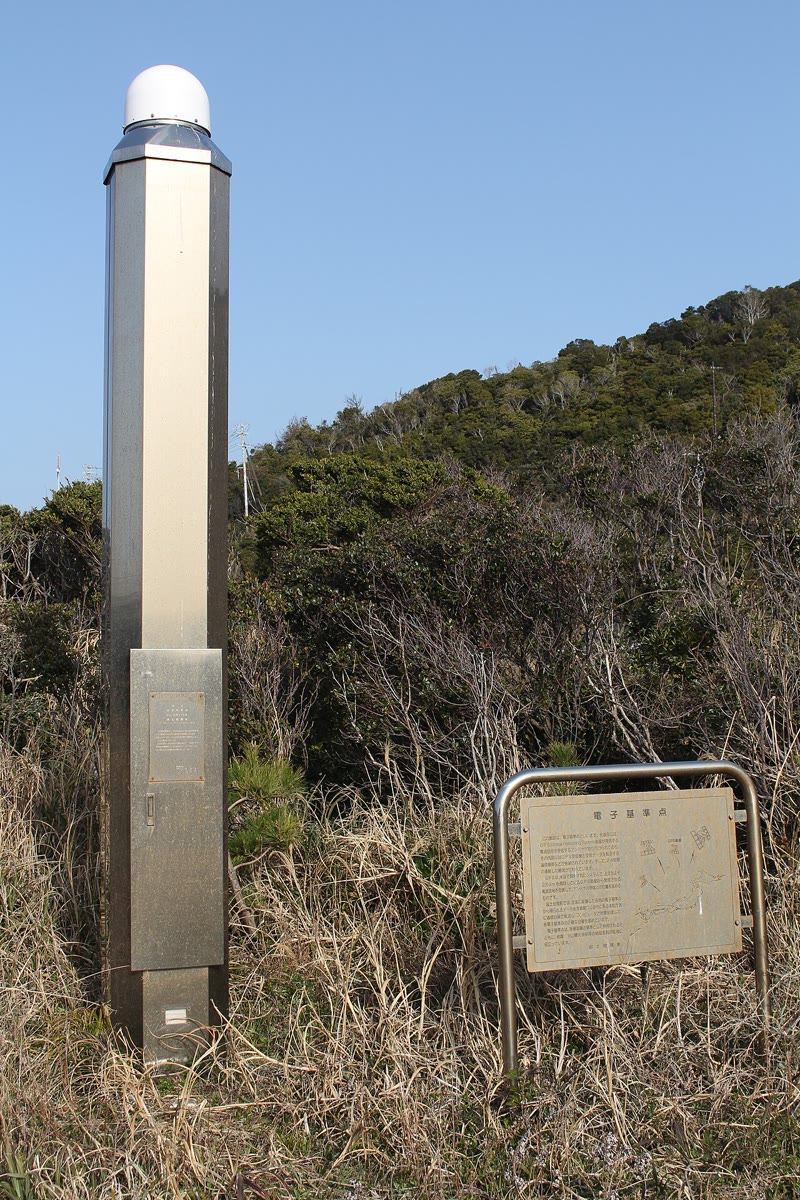
\includegraphics[width=\linewidth]{images/book3/b1-gnss-station.jpg}

{\scriptsize Une station permanente au Japon, son antenne sous le dôme
(Alpsdake, CC BY-SA 4.0).}
\end{minipage}
\end{inthefield}

Les vitesses de stations à l'intérieur de deux plaques donnent un \omterm{def:b1:plate-kinematics:euler-pole}{vecteur d'Euler}
qui leur est propre, indépendant de l'enregistrement géologique. Pour l'Eurasie par rapport à
l'Amérique du Nord, un tel vecteur prédit \qty{17.0}{mm.an^{-1}} en Islande, environ
\qty{8}{\percent} de moins que les \qty{18.6}{mm.an^{-1}} moyennés sur
\qty{3.16}{\Ma} (figure ci-dessus). La corde entre Reykjavik et Stavanger, toutes deux
sur des parties \omterm{def:b1:plate-kinematics:triple-junction}{stables} de leurs plaques, s'allonge de \qty{17.5}{mm.an^{-1}}~; le
vecteur issu des satellites prédit \qty{17.1}{mm.an^{-1}}, le géologique
\qty{18.6}{mm.an^{-1}}. À travers l'Atlantique nord, une vitesse mesurée sur quelques
décennies et une vitesse moyennée sur trois millions d'années s'accordent donc à
un dixième près~: là, les plaques se déplacent aujourd'hui presque comme elles se sont déplacées
pendant des millions d'années.
% ledger: morvel:gps-eu-na, morvel:eu-na, ngl:reyk, ngl:stas (chord rates computed in calc/ch12.py)

À l'intérieur de la zone de limite l'image est moins simple, car les stations bougent
avec plus que les plaques. Plus d'un dixième de l'Islande est sous des calottes glaciaires, et
la plupart perdent de la masse depuis environ 1890~: la \omterm{def:b1:layered-earth:layers}{croûte} en dessous se soulève à mesure que
la charge diminue, et se déplace horizontalement en s'éloignant de la glace qui s'amincit. La
station de Höfn, sur la côte sud-est près de la plus grande calotte, s'élève de
\qty{12.9}{mm.an^{-1}}.
% ledger: spaans:iceland-gia, ngl:hofn

\section{Exercices}

Prendre $R = \qty{6371}{km}$ dans tout ce qui suit.

\begin{exercise}[$\star$]\label{exo:b1:plate-kinematics:1}
Le \omterm{def:b1:plate-kinematics:euler-pole}{vecteur d'Euler} de l'Eurasie par rapport à l'Amérique du Nord a pour vitesse
\qty{0.210}{\degree\per\Ma}. (a) La convertir en \unit{rad.an^{-1}} et en
\unit{rad.s^{-1}}. (b) Combien de temps durerait un tour complet~? (c) Calculer $\omega R$ en
\unit{mm.an^{-1}}.
% ledger: morvel:eu-na
\end{exercise}

\begin{exercise}[$\star$]\label{exo:b1:plate-kinematics:2}
Avec le même \omterm{def:b1:plate-kinematics:euler-pole}{vecteur d'Euler}, calculer la vitesse relative des deux plaques à
\ang{30}, \ang{60} et \ang{90} du \omterm{def:b1:plate-kinematics:euler-pole}{pôle d'Euler}. Où le long de la limite de
plaques l'expansion serait-elle la plus rapide~?
\end{exercise}

\begin{exercise}[$\star$]\label{exo:b1:plate-kinematics:3}
Le sous-chron normal de Jaramillo a duré de \qty{1.072}{Ma} à \qty{0.988}{Ma}.
(a) Quelle est la largeur de la bande qu'il forme sur chaque flanc d'une dorsale de
\omterm{def:b1:plate-kinematics:spreading-rate}{demi-vitesse d'expansion} \qty{50}{mm.an^{-1}}~? De \qty{10}{mm.an^{-1}}~? (b) Quelle est la
largeur totale de la bande du chron normal actuel, qui a commencé
il y a \qty{0.781}{Ma}, sur une dorsale de demi-vitesse \qty{10}{mm.an^{-1}}~?
% ledger: iodp:gpts2004
\end{exercise}

\begin{exercise}[$\star$]\label{exo:b1:plate-kinematics:4}
Sur un profil à travers une dorsale, le bord jeune de l'anomalie du chron C2An,
âgé de \qty{2.581}{Ma}, se trouve à \qty{66}{km} à l'ouest de l'axe et à \qty{64}{km} à l'est
de celui-ci. Calculer les deux \omterm{def:b1:plate-kinematics:spreading-rate}{demi-vitesses d'expansion} et la \omterm{def:b1:plate-kinematics:spreading-rate}{vitesse totale d'expansion}.
L'expansion est-elle symétrique~?
% ledger: iodp:gpts2004
\end{exercise}

\begin{exercise}[$\star\star$]\label{exo:b1:plate-kinematics:5}
Un point de la dorsale de Gakkel, dans l'océan Arctique, se trouve à \ang{85}\,N, \ang{0}\,E.
Calculer sa distance angulaire au \omterm{def:b1:plate-kinematics:euler-pole}{pôle d'Euler} Eurasie--Amérique du Nord
(\ang{61.8}\,N, \ang{139.6}\,E, \qty{0.210}{\degree\per\Ma}) et la vitesse d'expansion
en ce point. Comparer aux vitesses mesurées de \qtyrange{11}{12}{mm.an^{-1}}.
% ledger: morvel:eu-na
\end{exercise}

\begin{exercise}[$\star\star$]\label{exo:b1:plate-kinematics:6}
Au \omterm{def:b1:plate-kinematics:triple-junction}{point triple} des Açores, \ang{39.44}\,N, \ang{29.83}\,O, calculer (a) la
distance angulaire au \omterm{def:b1:plate-kinematics:euler-pole}{pôle d'Euler} Eurasie--Amérique du Nord, (b) la vitesse
d'expansion, et (c) l'\omterm{def:b1:spherical-astronomy:horizontal}{azimut} du mouvement relatif. (d) Quelle orientation
prédit-on pour les failles transformantes de la dorsale juste au nord du \omterm{def:b1:plate-kinematics:triple-junction}{point triple}~?
% ledger: morvel:eu-na, morvel:azores
\end{exercise}

\begin{exercise}[$\star\star$]\label{exo:b1:plate-kinematics:7}
(a) Écrire les \omterm{def:b1:plate-kinematics:euler-pole}{vecteurs d'Euler} $\vec\omega_{\mathrm{EU\,NA}}$ (\ang{61.8}\,N,
\ang{139.6}\,E, \qty{0.210}{\degree\per\Ma}) et $\vec\omega_{\mathrm{NB\,NA}}$
(\ang{79.2}\,N, \ang{40.2}\,E, \qty{0.233}{\degree\per\Ma}) en composantes
cartésiennes, en \unit{\degree\per\Ma}. (b) En déduire $\vec\omega_{\mathrm{NB\,EU}}$,
son pôle et sa vitesse. (c) Pourquoi est-ce la meilleure façon de connaître le mouvement de la Nubie
par rapport à l'Eurasie~?
% ledger: morvel:eu-na, morvel:nb-na
\end{exercise}

\begin{exercise}[$\star\star$]\label{exo:b1:plate-kinematics:8}
Soit $\vec e_x$ dirigé vers \ang{0}\,N, \ang{0}\,E, $\vec e_y$ vers \ang{0}\,N,
\ang{90}\,E et $\vec e_z$ vers le pôle nord. Avec la formule de Rodrigues, calculer
l'image de $\vec e_x$ (a) par la rotation de \ang{90} autour de $\vec e_z$
suivie de la rotation de \ang{90} autour de $\vec e_x$~; (b) par les deux mêmes
rotations dans l'ordre inverse. (c) Qu'est-ce que cela signifie pour la
reconstruction des positions passées d'une plaque~?
\end{exercise}

\begin{exercise}[$\star\star$]\label{exo:b1:plate-kinematics:9}
Trois plaques A, B et C se rencontrent en un \omterm{def:b1:plate-kinematics:triple-junction}{point triple} dorsale--dorsale--dorsale.
Par rapport à A, la plaque B se déplace à \qty{30}{mm.an^{-1}} vers l'est et la plaque C à
\qty{40}{mm.an^{-1}} vers le sud. (a) Dessiner le triangle des vitesses.
(b) Calculer la vitesse et l'\omterm{def:b1:spherical-astronomy:horizontal}{azimut} de C par rapport à B. (c) Quelle est l'orientation de
la dorsale entre B et C si elle s'ouvre perpendiculairement à son axe~?
\end{exercise}

\begin{exercise}[$\star\star\star$]\label{exo:b1:plate-kinematics:10}
(a) Montrer que la trace de la matrice $R$ d'une rotation d'angle $\alpha$ autour d'un axe quelconque
est $1 + 2\cos\alpha$. (b) La matrice
\[
  R = \begin{pmatrix} 0 & 0 & 1\\ 1 & 0 & 0\\ 0 & 1 & 0\end{pmatrix}
\]
est orthogonale de déterminant $1$. Trouver son axe, sous forme d'une \omterm{def:b1:spherical-astronomy:geographic}{latitude} et d'une \omterm{def:b1:spherical-astronomy:geographic}{longitude},
et son angle. (c) Vérifier votre réponse en appliquant $R$ à $\vec e_x$, $\vec e_y$
et $\vec e_z$.
\end{exercise}

\begin{exercise}[$\star\star\star$]\label{exo:b1:plate-kinematics:11}
Avant le positionnement par satellite, les \omterm{def:b1:plate-kinematics:euler-pole}{pôles d'Euler} étaient trouvés à partir des orientations de
failles transformantes. (a) Montrer que le \omterm{def:b1:plate-kinematics:euler-pole}{pôle d'Euler} se trouve sur le \omterm{def:b1:spherical-astronomy:spherical-triangle}{grand cercle} passant par
un point d'une faille transformante et perpendiculaire à la faille en ce point, et que
le pôle est donc selon $\vec t_1\times\vec t_2$, où $\vec t_1$ et
$\vec t_2$ sont des vecteurs unitaires le long de deux failles transformantes de la même limite.
(b) Des failles transformantes sont orientées à \ang{95} près du \omterm{def:b1:plate-kinematics:triple-junction}{point triple} des Açores
(\ang{39.44}\,N, \ang{29.83}\,O) et à \ang{103} en Islande (\ang{64.5}\,N,
\ang{18}\,O). Le vecteur unitaire horizontal à la \omterm{def:b1:spherical-astronomy:geographic}{latitude} $\varphi$ et à la \omterm{def:b1:spherical-astronomy:geographic}{longitude}
$\lambda$ pointant vers l'\omterm{def:b1:spherical-astronomy:horizontal}{azimut} $\beta$ est $\sin\beta\,\vec e +
\cos\beta\,\vec n$, avec $\vec e = (-\sin\lambda, \cos\lambda, 0)$ et $\vec n =
(-\sin\varphi\cos\lambda, -\sin\varphi\sin\lambda, \cos\varphi)$. Localiser le
pôle. (c) Avec quelle précision deux transformantes déterminent-elles le pôle~?
% ledger: morvel:eu-na
\end{exercise}

\begin{exercise}[$\star\star\star$]\label{exo:b1:plate-kinematics:12}
La position vers l'est d'une station, tous les trois mois pendant trois ans, est
(en millimètres, à partir de $t = 0$)~:
\begin{center}\small
\begin{tabular}{l*{13}{c}}
\hline
$t$ (ans) & 0 & 0.25 & 0.5 & 0.75 & 1 & 1.25 & 1.5 & 1.75 & 2 & 2.25 & 2.5 & 2.75 & 3\\
$x$ (mm) & 4 & 5 & 6 & 15 & 24 & 25 & 26 & 65 & 74 & 75 & 76 & 85 & 94\\
\hline
\end{tabular}
\end{center}
Elle est faite d'un mouvement régulier, d'une oscillation saisonnière et d'un saut dû à un
séisme. (a) Calculer la vitesse à partir de la première et de la dernière position.
(b) Calculer les neuf différences entre positions distantes d'exactement un an, et
leur médiane. (c) Expliquer pourquoi la médiane des différences à un an est une estimation robuste
de la vitesse régulière, et quand elle échouerait.
\end{exercise}

\section{Problème~: L'Islande se fend}

\begin{problem}[{Problème du week-end --- l'ouverture de l'Atlantique nord à travers
l'Islande, mesurée de trois façons}]
\label{pb:b1:plate-kinematics:1}
% values: calc/ch12.py (Part II profile invented for the problem; real Euler
% vectors, chron ages and station velocities)
% ledger: morvel:eu-na, morvel:nb-na, iodp:gpts2004, ngl:reyk, ngl:stas, ngl:hofn
L'Islande se trouve sur la dorsale médio-atlantique, entre la plaque nord-américaine à
l'ouest et la plaque eurasienne à l'est. Prendre $R = \qty{6371}{km}$ et, pour
l'Eurasie par rapport à l'Amérique du Nord, le \omterm{def:b1:plate-kinematics:euler-pole}{vecteur d'Euler} de pôle
\ang{61.8}\,N, \ang{139.6}\,E et de vitesse \qty{0.210}{\degree\per\Ma}.

\medskip
\noindent\textbf{Partie I --- Le vecteur des plaques.}
\begin{enumerate}
  \item Convertir la vitesse en \unit{rad.an^{-1}} et calculer $\omega R$ en
        \unit{mm.an^{-1}}.
  \item Calculer la distance angulaire $\Delta$ du pôle au centre de
        l'Islande, \ang{64.5}\,N, \ang{18}\,O.
  \item En déduire la \omterm{def:b1:plate-kinematics:spreading-rate}{vitesse totale d'expansion} à travers l'Islande prédite par le vecteur
        des plaques.
  \item Calculer l'\omterm{def:b1:spherical-astronomy:horizontal}{azimut} du pôle vu depuis l'Islande, et l'\omterm{def:b1:spherical-astronomy:horizontal}{azimut} du
        mouvement de l'Eurasie par rapport à l'Amérique du Nord.
  \item Décomposer cette vitesse en ses composantes est et nord.
  \item Sur la dorsale de Gakkel, à \ang{86}\,N, \ang{60}\,E, quelle vitesse donne le même
        vecteur~? Pourquoi la limite y est-elle tellement plus lente~?
\end{enumerate}

\noindent\textbf{Partie II --- Les bandes magnétiques.}
Un profil magnétique de navire à travers la dorsale de Reykjanes, au sud-ouest de l'Islande près de
\ang{63}\,N, \ang{23}\,O, mené dans la direction de l'expansion, donne les distances suivantes
de l'axe à trois limites de chrons (un profil construit pour
ce problème)~:
\begin{center}\small
\begin{tabular}{lccc}
\hline
limite & âge (Ma) & à l'ouest de l'axe (km) & à l'est de l'axe (km)\\
\hline
base de C1n & 0.781 & 9.7 & 10.1\\
bord jeune de C2An & 2.581 & 26.8 & 27.3\\
bord jeune de C5n & 9.779 & 94 & 97\\
\hline
\end{tabular}
\end{center}
\begin{enumerate}[resume]
  \item À partir du bord jeune de C5n, calculer les deux \omterm{def:b1:plate-kinematics:spreading-rate}{demi-vitesses d'expansion}.
  \item En déduire la \omterm{def:b1:plate-kinematics:spreading-rate}{vitesse totale d'expansion} depuis \qty{9.8}{Ma}.
  \item Calculer aussi la vitesse totale à partir des deux limites plus jeunes. Les
        trois s'accordent-elles~? Décrire comment elles changent avec l'âge de la limite.
  \item L'expansion est-elle symétrique~? L'asymétrie change-t-elle la vitesse totale~?
  \item Sur la dorsale de Reykjanes, les limites entre bandes sont déplacées
        loin de l'axe de \qty{5.0}{km} en tout, les deux flancs ensemble.
        Corriger les trois vitesses totales. Pourquoi la correction a-t-elle compté le plus pour
        la limite la plus jeune~?
  \item Quelle est la largeur de la bande du sous-chron de Jaramillo
        (\qtyrange{1.072}{0.988}{Ma}) sur chaque flanc, à la demi-vitesse
        corrigée~? La comparer au déplacement de la question 11. L'anomalie de
        Jaramillo est pourtant nettement reconnue sur les profils de la dorsale de Reykjanes,
        mais est absente de la dorsale de Gakkel~: qu'est-ce que cela suggère~?
  \item Le vecteur des plaques prédit \qty{19.0}{mm.an^{-1}} au profil. Comparer
        avec vos vitesses corrigées.
\end{enumerate}

\noindent\textbf{Partie III --- Les satellites.}
Les stations permanentes REYK (Reykjavik, \ang{64.139}\,N, \ang{21.955}\,O) et
STAS (Stavanger, \ang{59.018}\,N, \ang{5.599}\,E) se trouvent sur les plaques nord-américaine et
eurasienne. Leurs vitesses mesurées font que la corde qui les joint s'allonge
de \qty{17.5}{mm.an^{-1}}.
\begin{enumerate}[resume]
  \item Calculer la distance angulaire entre les deux stations, et la longueur
        de la corde.
  \item Combien de temps la corde met-elle à s'allonger d'un mètre~?
  \item Le vecteur des plaques donne à STAS une vitesse de \qty{18.9}{mm.an^{-1}} vers
        \ang{114.8} par rapport à l'Amérique du Nord. Le \omterm{def:b1:spherical-astronomy:spherical-triangle}{grand cercle} issu de REYK
        arrive à STAS en cap vers \ang{123.1}. Calculer la composante de
        la vitesse le long de cette direction, puis l'allongement prédit de
        la corde, qui fait l'angle $\Delta/2$ avec l'horizontale à STAS.
  \item Comparer l'allongement mesuré et l'allongement prédit. Qu'est-ce qui pourrait expliquer
        la différence~?
  \item Par rapport à l'Amérique du Nord, REYK se déplace à \qty{1.07}{mm.an^{-1}} vers
        l'ouest et \qty{0.97}{mm.an^{-1}} vers le sud, et la station HOFN (Höfn,
        sud-est de l'Islande) à \qty{21.12}{mm.an^{-1}} vers l'est et
        \qty{6.97}{mm.an^{-1}} vers le sud. Calculer la vitesse et l'\omterm{def:b1:spherical-astronomy:horizontal}{azimut} de HOFN
        par rapport à REYK.
  \item Comparer avec la partie I. HOFN s'élève aussi de \qty{12.9}{mm.an^{-1}}. Pourquoi les
        stations situées à l'intérieur de l'Islande sont-elles une mauvaise mesure du mouvement des plaques~?
\end{enumerate}

\noindent\textbf{Partie IV --- Dix millions d'années, et le point triple au sud.}
\begin{enumerate}[resume]
  \item Sur \qty{10}{\Ma}, de quel angle l'Eurasie tourne-t-elle par rapport à
        l'Amérique du Nord autour du pôle~?
  \item Quelle distance un point de l'Eurasie au milieu de l'Islande parcourt-il le long de
        son \omterm{def:b1:spherical-astronomy:spherical-triangle}{petit cercle} pendant ce temps~? La comparer à la largeur corrigée de la
        \omterm{def:b1:layered-earth:layers}{croûte} formée depuis le bord jeune de C5n dans la partie II.
  \item Au \omterm{def:b1:plate-kinematics:triple-junction}{point triple} des Açores, les vecteurs des plaques donnent à l'Eurasie
        \qty{22.9}{mm.an^{-1}} vers \ang{95.1} et à la Nubie
        \qty{19.2}{mm.an^{-1}} vers \ang{103.8}, tous deux par rapport à l'Amérique du
        Nord. Calculer la vitesse de l'Eurasie par rapport à la Nubie.
  \item Ce \omterm{def:b1:plate-kinematics:triple-junction}{point triple} est-il \omterm{def:b1:plate-kinematics:triple-junction}{stable}~? Quel type de limite la vitesse de la
        question 22 implique-t-elle entre l'Eurasie et la Nubie~?
  \item Rassembler les vitesses d'ouverture des parties I, II et III. Lesquelles s'accordent, et
        quelle méthode mesure le mouvement des plaques sur la durée la plus courte~?
  \item Au millimètre par an près, quelle \omterm{def:b1:plate-kinematics:spreading-rate}{vitesse totale d'expansion} à travers
        l'Islande donnent à la fois le vecteur des plaques et les bandes magnétiques
        corrigées~?
\end{enumerate}
\end{problem}
